
\chapter{Einschränkung der Kopplungsparameter durch Supernovae}

Im Folgenden betrachten wir einige der Argumente, die genutzt werden können, um die Kopplungsparameter zwischen Majoronen und Neutrinos einzuschränken, näher.
Konkret gehen wir auf die Einschränkungen durch Neutrinospektren ein, die es uns ermöglichen, die Kopplungsparameter $g_1$ und $g_2$ einzuschränken, und die Einschränkungen aus der Majoronenluminosität ein,
die uns eine Ausschlussregion für $|\tilde{g}_{i j}|$ liefert.
Zusätzlich wird kurz das aktuelle Limit auf die Neutrinomasse $m_1$ diskutiert.

\section{Grenzen durch Neutrinospektren}
\label{subsec:spektrengrenzen}

Durch Majoronen induzierte Flavourübergänge der Neutrinos der Form $\tilde{\nu}^\pm_i \rightarrow \tilde{\nu}^\mp_j + J$ können das Energiespektrum der einzelnen Neutrinogenerationen merklich verschieben. 
Dabei muss jedoch beachtet werden, dass die Wirkungsquerschnitte der unterschiedlichen Neutrinos innerhalb einer typischen Supernova nicht übereinstimmen.
Diese Diskrepanz stammt daher, dass $\nu_\mu$ und $\nu_\tau$ nur über neutrale Ströme mit dem Supernovamedium interagieren können.
Innerhalb von Supernovae verhalten $\nu_\mu$ und $\nu_\tau$ sich also nahezu gleich.
Elektronneutrinos $\nu_e$ können dagegen nicht nur über neutrale, sondern auch über geladene Ströme mit dem Medium wechselwirken.
So können sie unter Abstrahlung eines $W$-Bosons mit den im Überfluss vorhandenen Elektronen interagieren, während Wechselwirkungen von $\nu_\mu$ und $\nu_\tau$ mit der Materie in den dichteren Regionen des sterbenden Sterns kaum zustande kommen.
Es entsteht also ein Spektrum niedrigerer Temperaturen für $\nu_e$ und höherer Temperaturen für $\nu_\mu$ und $\nu_\tau$, dass durch Neutrinozerfälle verzerrt werden kann.
Berücksichtigen wir nun zusätzlich zur Zerfallswahrscheinlichkeit $N_\text{decay}$ außerdem die Oszillationswahrscheinlichkeit $N_\text{osc}$ der Neutrinos nach dem Verlassen seiner Energiesphäre mit Radius $R_{E, \tilde{\nu}^\pm_i}$, 
bis sie hier auf der Erde ankommen, lässt sich die effektive Wahrscheinlichkeit, dass ein Neutrino mit seinem ursprünglichen Flavour die Erde erreicht, als
\begin{equation}
    N = N_\text{decay} \cdot N_\text{osc}
    \label{eq:survivalprob}
\end{equation}
schreiben \cite{supernovaboundsdasandere}.

Die Zerfallswahrscheinlichkeit ist dabei gegeben durch
\begin{equation}
    N_\text{decay}(\tilde{\nu}^\pm) \cong \exp \left(- \int^\infty_{R_{E, \tilde{\nu}^\pm_i}} \mathrm{d}r \, \sum_j \Gamma(\tilde{\nu}^\pm_i \rightarrow \tilde{\nu}^\mp_j + J) \right) \,.
    \label{eq:zerfallswkeit}
\end{equation}
In relativistischer Näherung, die wir hier bereits zur Bestimmung der Materieeigenzustände verwendet haben, lässt sich die Zerfallsrate $\Gamma(\tilde{\nu}^\pm_i \rightarrow \tilde{\nu}^\mp_j + J)$ durch
\begin{equation}
    \Gamma(\tilde{\nu}^\pm_i \rightarrow \tilde{\nu}^\mp_j + J) = \frac{|\tilde{g}^2_{i j}|}{16 \pi} \left(V_i - V_f \right)
    \label{eq:zerfallsrate}
\end{equation}
ausdrücken, wobei $V_i - V_f$ die Potentialdifferenz zwischen Anfangs- und Endzustand beschreibt.

Die Oszillationswahrscheinlichkeit hängt stark von der gewählten Massendifferenz und dem Mischungswinkel zwischen den Neutrinos ab.
Wir fokussieren uns hier auf die LMA-MSW, also die Large-Mixing-Angle MSW-Lösung, die einen großen Mischungswinkel annimmt.
Wie in \cite{ueberlebenswkeit} genauer erläutert ergibt sich so eine Oszillationswahrscheinlichkeit von
\begin{equation}
    N_\text{osc} = 1 - \left[\sin^2\theta_\odot - \sin 2\theta_m \sin\left(2\theta_\odot - 2 \theta_m\right) \sin^2 \left(\frac{\pi d}{l_m}\right)\right] \,,
    \label{eq:osziwkeit}
\end{equation}
wobei
\begin{equation*}
    l_m = \frac{4 \pi E}{\Delta m^2_\odot} \frac{\sin2\theta_m}{\sin2\theta_\odot}
\end{equation*}
die Oszillationslänge und $\theta_m$ den Mischungswinkel der Neutrinos in Materie, die sie auf einer Distanz $d$ in der Erde bis zum Detektor durchdringen, beschreibt.
Durch die Näherung $\theta_{1 3} = 0$ gehen wir davon aus, dass es nur zu einer Mischung zwischen Elektron- und Myonneutrinos kommt, der Mischungswinkel $\theta_m$ lässt sich also mit $\theta_\odot$ identifizieren.
So lassen sich, wenn wir, wie in \cite{supernovaboundsdasandere} gezeigt, die entsprechenden, fehlenden Größen in \eqref{eq:osziwkeit} einsetzen, die Kopplungsparameter $g_1$ und $g_2$ auf einige $10^{-4}$ einschränken.

\section{Grenzen durch Majoronenluminosität}

Um die Grenzen auf die Kopplungsparameter $|g_{i j}|$ aus der Majoronenluminosität zu erhalten, betrachten wir das Neutrinosignal der Supernova SN$1987$A unter der Annahme, dass $\nu_e$ nur geringfügig mit den anderen Flavours mischt.
Unter dieser Annahme passt das beobachtete Neutrinosignal gut zu numerischen Berechnungen der totalen Bindungsenergien in einer Supernova und erlaubt es uns, eine Ausschlussregion von auf die Kopplungsparameter durch
\begin{equation}
    3 \cdot 10^{-7} < |g_{i j}| < 2 \cdot 10^{-5} %%%%%%%%%%%%%%% TEMP!!!! AKTUALISIERUNG MIT DEN NEUEN DATEN. PÄS BITTE ANTWORTE MIIIIIR
    \label{eq:gijlimit}
\end{equation}
festzulegen.

Lägen die Kopplungen in dem ausgeschlossenen Bereich, würden wir eine merkliche Unterdrückung der beobachteten Energie erwarten.
Für Werte $|g_{i j}| < 3 \cdot 10^{-7}$ wird die Kopplung zwischen Neutrinos und Majoronen so schwach, das kein merklicher Effekt auf das Supernovaspektrum entstehen würde. %%%% HIER SIND AUCH NOCH ALTE LIMITS!
Auf der anderen Seite wird die Kopplung für $|g_{i j}| > 2 \cdot 10^{-5}$ so stark, dass die Majoronen das Innere der Supernova nicht länger verlassen könnten. %%%% HIER SIND AUCH NOCH ALTE LIMITS!
So würden sie ebenfalls nicht zu einer Änderung des Energiespektrums beitragen.


\section{Neutrinomassengrenze aus KATRIN}
\label{subsec:KATRIN}

Das KATRIN-Experiment in Karlsruhe ist in der Lage, die Masse des Elektronneutrinos stark einzuschränken.
Dies ist möglich, indem das kontinuierliche Energiespektrum der Elektronen beim $\beta$-Zerfall genauestens untersucht wird, genauer genommen das Abknicken dieses Spektrums für die maximale Elektronenenergie.
Dieser Knick ist näher in \autoref{fig:elektronenspektrum} dargestellt.
\begin{figure}[H]
    \centering
    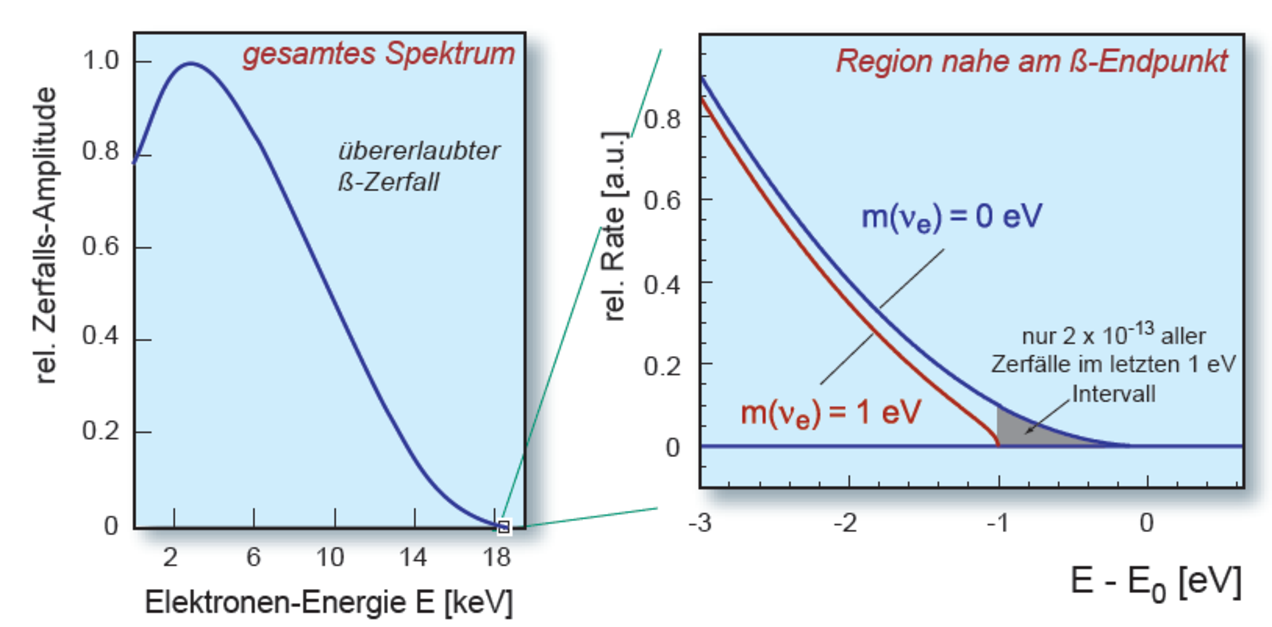
\includegraphics[width=.5\textwidth]{figures/Elektronenspektrum.pdf}
    \caption{Spektrum der Elektronen beim $\beta$-Zerfall. Die linke Kurve zeigt das gesamte Spektrum von der minimalen bis zur maximalen Energie, die das Elektron während des Zerfalls erhält. Rechts
            ist hochenergetische Ende der Kurve vergrößert dargestellt. Es wird ein Vergleich zwischen dem Kurvenverlauf unter der Annahme eines masselosen Neutrinos $m(\nu_e) = 0$ und dem Kurvenverlauf unter Freisetzung
            eines Elektronneutrinos mit einer Masse von $1 \si{\eV}$ hergestellt. Charakteristisch ist das Abknicken der Kurve für $m(\nu_e) \neq 0$. Dieses Abknicken stammt daher, dass das Elektron nicht länger
            die maximale Stoßenergie besitzen kann, sobald das Neutrino Masse besitzt \cite{elektronenspektrum}.}
    \label{fig:elektronenspektrum}
\end{figure}
Durch die Analyse der Position dieses Knicks konnte die Neutrinomasse Anfang $2022$ auf $m_1 < \SI{0.8}{\eV}$ \cite{KATRINneutrinogrenze} eingeschränkt werden.
Gemeinsam mit den in \autoref{subsec:spektrengrenzen} gefundenen Einschränkungen auf $g_1$ und damit auch auf $g_2$ lässt sich so das Fenster wählen, in dem die erstellten Plots relevant sind.



\section{Ausschlussregionen der Kopplungsparameter}

Mit den bisher zusammengestellten Einschränkungen auf $g_i$ und $m_1$ ist es uns, gemeinsam mit der Ausschlussregion auf $|g_{i j}|$ möglich, Grafiken zu erstellen, die uns die zulässigen Bereiche für $g_1$ und $m_1$ deutlich machen.
Dazu betrachten wir die einzelnen Einträge in \eqref{eq:materiekoppmat} und nutzen die Ausdrücke in \eqref{eq:g2g3}, um $|g_{i j}|$ nur in Abhängigkeit von $g_1$ und $m_1$ zu schreiben.
Somit ist es uns möglich, anschließend wahlweise $g_1$ in Abhängigkeit von $m_1$ oder $m_1$ in Abhängigkeit von $g_1$ auszudrücken.
Hier entscheiden wir uns für $m_1 (g_1)$, um einen besseren Vergleich zu \cite{päspaper} herstellen zu können.
Für alle folgenden Plots werden die LMA-MSW-Werte
\begin{align}
    \sin^2\theta_\odot = \num{0.307}\,, && \Delta m^2_\odot = \num{7.53} \cdot 10^{-5} \si{eV}^2\,, && \Delta m^2_\text{atm} = \num{2.453} \cdot 10^{-3} \si{\eV}^2
    \label{eq:LMAMSW}
\end{align}
verwendet \cite{neutrinospdg}.

Beginnen wir zunächst mit der Kopplung $g_{ee}$.
Hier gehen wir die Rechnung einmal Schritt für Schritt durch, da die Rechenschritte allerdings nur aus Umformungen und trivialen Operationen besteht und für alle Kopplungen dem gleichen Schema folgt, werden wir auf die Berechnungen der anderen
Kopplungen nicht näher eingehen.

Wie in \eqref{eq:materiekoppmat} zu erkennen ist, gilt
\begin{equation}
    g_{ee} = g_1 \cos^2 \theta_\odot + g_2 \sin^2 \theta_\odot \mathrm{e}^{-2 i \delta} \,.
    \label{eq:g_ee}
\end{equation}
Unter der Nutzung von
\begin{equation*}
    g_2 = g_1 \sqrt{1 + \frac{\Delta m^2_\odot}{m^2_1}}
\end{equation*}
aus \eqref{eq:g2g3} erhalten wir
\begin{equation*}
    g_1 \sqrt{1 + \frac{\Delta m^2_\odot}{m^2_1}} = \frac{g_{ee} - g_1 \cos^2 \theta_\odot}{\sin^2 \theta_\odot} \mathrm{e}^{2 i \delta} \,.
\end{equation*}
Dividieren wir durch $g_1$, quadrieren die gesamte Gleichung und bringen die $1$ auf die andere Seite, erhalten wir
\begin{equation*}
    \frac{\Delta m^2_\odot}{m^2_1} = \left(\frac{g_{ee} -  \cos^2 \theta_\odot \, g_1}{\sin^2 \theta_\odot \, g_1} \mathrm{e}^{2 i \delta} \right)^2 - 1 \,.
\end{equation*}
Jetzt müssen wir nur noch den Kehrwert bilden.
Dann ist durch die Wurzel der Gleichung das Ergebnis
\begin{equation}
    m_1 = \sqrt{\frac{\Delta m^2_\odot}{\left(\frac{g_{ee} -  \cos^2 \theta_\odot \, g_1}{\sin^2 \theta_\odot \, g_1} \mathrm{e}^{2 i \delta} \right)^2 - 1}}
    \label{eq:m_1g_ee}
\end{equation}
gegeben.

Da die CP-verletzende Phase $\delta$ frei wählbar ist, wählen wir hier zur Darstellung der Kopplung stets die beiden Extreme $\delta = 0$, also einen maximal positiven, und $\delta = \frac{pi}{2}$, also einen maximal negativen Phasenbeitrag.
An \eqref{eq:m_1g_ee} wird aber schnell erkennbar, dass genau diese Wahl der Phasen keinerlei Auswirkungen auf die Parametrisierung von $m_1$ zu haben scheint.
Denn mit $\mathrm{e}^{2 i \frac{\pi}{2}} = -1$ wird das negative Vorzeichen durch das Quadrat wieder aufgehoben.
Wir sehen aber, dass die gewählte Phase zumindest für die Bestimmung des durch die in \autoref{subsec:KATRIN} erläuterte Massengrenze auftretenden Cutoff nicht ganz irrelevant ist.

Um genau diesen Cutoff an der Massengrenze zu ermitteln, stellen wir \eqref{eq:g_ee} außerdem nach $g_1$ statt $m_1$ um, erhalten
\begin{equation}
    g_1 = \frac{g_{ee}}{\cos^2\theta_\odot + \sqrt{1 + \frac{\Delta m^2_\odot}{m^2_1}} \sin^2\theta_\odot \mathrm{e}^{-2 i \delta}} 
    \label{eq:g1cutoffg_ee}
\end{equation}
und setzen für $m_1$ schließlich das gewünschte Limit ein.
Der Cutoff der anderen Kopplungen folgt dem gleichen Prinzip, darauf wollen wir hier aufgrund der Trivialität der Rechnungen nicht näher eingehen.
Wählen wir $m_1 \gg \Delta m^2_\odot$, beeinflusst die Wahl von $m_1$ nicht länger das Ergebnis von $g_1$ und es entsteht das in \autoref{fig:m_1g_ee} erkennbare divergente Verhalten.
Hier ist die Phasenabhängigkeit offensichtlich.
Wählen wir eine Phase von $\delta = \frac{\pi}{2}$ ist es möglich, dass sich die beiden Terme in \eqref{eq:g1cutoffg_ee} gegenseitig eliminieren.
So entstehen zwei Zweige, die an unterschiedlichen Stellen nahezu parallel zur $y$-Achse $m_1 = \SI{0.8}{\eV}$ erreichen.
Dazu sei gesagt, dass, da sie die Einschränkung von $|g_{i j}|$ nur auf den Betrag beziehen, immer vier Kurven, jeweils zwei für die positiven und zwei für die negativen Ober- und Untergrenzen entstehen.
%\begin{figure}[H]
%    \centering
%    \includegraphics[width=0.8\textwidth]{build/m1g1g_ee.pdf}
%    \caption{Neutrinomasse $m_1$ in Abhängigkeit des Kopplungsparameters $g_1$ für $g_{ee}$. Die durchgezogenen blauen Linien stellen dabei die untere und obere Grenze $g_{ee} = 3 \cdot 10^{-7}$ bzw. $g_{ee} = 2 \cdot 10^{-5}$
%            mit einer Phase von $\delta = 0$, die gestrichelten Linien die Grenzen bei einer Phase von $\delta = \frac{\pi}{2}$ dar. Gemeinsam mit den türkisen Linien der negativen Grenzen auf $|g_{ee}|$ entsteht so die blau
%            gefüllte Ausschlussfläche. Die rote Fläche kennzeichnet dabei den durch KATRIN ausgeschlossen Massenbereich von $m_1 > \SI{0.8}{\eV}$.}
%    \label{fig:m_1g_ee}
%\end{figure}
Die Ausschlussregion ist dabei so gewählt, dass ein möglichst großer Parameterbereich übrig bleibt.
Hier werden also nur die innersten Kurven zur Bildung der Fläche verwendet.
Für einen bestimmten, relativ schmalen Wertebereich von $g_1$ wird in \eqref{eq:m_1g_ee} das quadrierte Argument im Nenner der Wurzel kleiner als 1.
Damit wird die Wurzel imaginär und es entsteht die beobachtbare Lücke im Plot.
Auffällig ist auch das asymptotische Verhalten der Äste für verhältnismäßig große $g_1$.
Wird $g_1$ groß gegen die gewählte Grenze von $g_{ee}$, gilt näherungsweise 
\begin{equation*}
    \frac{g_{ee} -  \cos^2 \theta_\odot \, g_1}{sin^2 \theta_\odot \, g_1} \mathrm{e}^{2 i \delta} \approx \frac{\cos^2 \theta_\odot \, g_1}{sin^2 \theta_\odot \, g_1} \mathrm{e}^{2 i \delta}
    = \frac{\cos^2 \theta_\odot}{sin^2 \theta_\odot} \mathrm{e}^{2 i \delta} \,.
\end{equation*}
In dem Fall ist $m_1$ also durch
\begin{equation*}
    m_1 (g_1) = \sqrt{\frac{\Delta m^2_\odot}{ \left(\frac{\cos^2 \theta_\odot}{\sin^2 \theta_\odot} \mathrm{e}^{2 i \delta}\right)^2 - 1}}
\end{equation*}
gegeben, $m_1$ ist also konstant. \\
Diese asymptotische Konvergenz gegen $m_1 \approx \num{4.2902} \cdot 10^{-3} \, \si{\eV}$ tritt für alle Werte von $g_{ee}$ früher oder später ein.

Analog gehen wir für die restlichen Kopplungen vor.
So ergibt sich aus
\begin{equation*}
    g_{e \mu'} = \frac{1}{2} \left(-g_1 + g_2 \mathrm{e}^{-2 i \delta}\right) \sin(2 \theta_\odot)
\end{equation*}
für die Kopplung $g_{e \mu'}$
\begin{equation}
    m_1 = \sqrt{\frac{\Delta m^2_\odot}{\left( \left(\frac{2 g_{e \mu'}}{\sin{2 \theta_\odot}} + 1 \right) \mathrm{e}^{2 i \delta}\right)^2 - 1}} \,.
    \label{eq:g_emu}
\end{equation}
Auch hier ist zu erkennen, dass $m_1$ sich für $\delta = 0$ und $\delta = \frac{\pi}{2}$ nicht unterscheidet.

Für $g_{\mu' \mu'}$ folgt aus
\begin{equation*}
    g_{\mu' \mu'} = g_1 \sin^2 \theta_\odot + g_2 \cos^2 \theta_\odot\mathrm{e}^{-2 i \delta}
\end{equation*}
\begin{equation}
    m_1 = \sqrt{\frac{\Delta m^2_\odot}{\left(\frac{g_{ee} -  \cos^2 \theta_\odot \, g_1}{\sin^2 \theta_\odot \, g_1} \mathrm{e}^{2 i \delta} \right)^2 - 1}} \,.
    \label{eq:m_1g_mumu}
\end{equation}
Da $g_{ee}$ und $g_{\mu' \mu'}$ bis auf ein Tauschen der Koeffizienten vor $\sin^2\theta_\odot$ und $\cos^2\theta_\odot$ vollständig übereinstimmen, weisen auch die Ausdrücke für $m_1$ große Ähnlichkeiten auf.
Ein Unterschied ist allerdings, dass alle vier Kurven $m_1$ für $g_{\mu \mu}$, im Gegenteil zu den Verläufen der oberen Grenzen von $m_1$ für $g_{ee}$, nur aus einem einzigen divergenten Zweig bestehen.

Schlussendlich folgt für $g_{\tau' \tau'}$ aus
\begin{equation*}
    g_{\tau' \tau'} = g_3 = g_1 \sqrt{1 + \frac{\Delta m^2_\odot + \Delta m^2_\text{atm}}{m^2_1}}
\end{equation*}
\begin{equation}
    m_1 = \sqrt{\frac{\Delta m^2_\odot + \Delta m^2_\text{atm}}{\left(\frac{g_{\tau' \tau'}}{g_1}\right)^2 - 1}} \,.
    \label{eq:g_tautau}
\end{equation}
Dieser Ausdruck für $m_1$ unterscheidet sich am stärksten von den anderen.
Das hat vor allem den Grund, dass wir hier annehmen, dass die Elektron- und Myonflavours nicht mit $\nu_\tau$ mischen, $g_{\tau' \tau'}$ also nur von der Kopplung der Tau-Neutrinos mit den Majoronen abhängt.

Gemeinsam entsteht so der in \autoref{fig:m_1all} dargestellte Plot.
Dabei haben wir für jede Kopplung $g_{i j}$ bereits die konservativste Ausschlussregion gewählt, sodass für jede Kopplung eine Kurve für die Untergrenze und eine Kurve für die Obergrenze übrigbleiben.
Alle restlichen Kurven werden aus dem Plot entfernt. 
\begin{figure}[H]
    \centering
    \includegraphics[width=.8\textwidth]{build/g_1m_1new.pdf}
    \caption{Grafische Repräsentation der unterschiedlichen Vorschriften für $m_1$ in Abhängigkeit des Kopplungsparameters $g_1$. Erneut werden die in \eqref{eq:LMAMSW} erwähnten LMA-Werte genutzt.
            Die dargestellten Kurven zeigen bereits eine Auswahl der konservativsten Ausschlussregionen, allerdings innerhalb einer Kopplung $g_{i j}$. 
            Die Kopplung $g_{e \mu'}$ wird auf den Schnittpunkt der Ober- und Untergrenze beschränkt.}
    \label{fig:m_1all}
\end{figure}
Hier lässt sich noch anmerken, dass sich alle Kurven für $g_1 \ll g_{i j}$ linear verhalten, hier $g_{i j}$ das Verhalten dominiert.

Damit lässt sich die gesamte Ausschlussregion als Zusammenschluss aller Einzelregionen darstellen, sodass sich \autoref{fig:finalplot} ergibt.
%\begin{figure}[H]
%    \centering
%    \includegraphics[width=.8\textwidth]{build/finalplot.pdf}
%    \caption{Finale Ausschlussregion durch Zusammenschluss der einzelnen Ausschlussregionen. Die Einhüllende der Untergrenze ist die Vorschrift für $m_1$ aus $g_{\tau' \tau'}$, 
%            die Obergrenze entsteht durch das Zusammenspiel aller Grenzen durch $g_{ee}$ und $g_{e \mu'}$. Die Einschränkungen durch $g_{\mu' \mu'}$ beeinflussen die resultierende Fläche nicht.}
%    \label{fig:finalplot}
%\end{figure}


